\section*{Appendices}\parskip=-1mm
\addcontentsline{toc}{section}{{\textbf{Appendices}}}

\vspace{8pt}

\subsection{Appendices 1: Further Information for proposed Testbed}

\vspace{8pt}

\begin{itemize}[leftmargin=0.1cm]
    % \setlength{\itemsep}{-0.1cm}
    \item \textbf{BLE Devices:} A variety of commercial BLE devices, such as sensors, locks, and beacons, which represent a cross-section of typical endpoints found in BLE networks. These devices are instrumental in generating the benign traffic patterns for our datasets.
    \item \textbf{User Devices:} Smartphones, tablets, and computers used by end-users to interact with BLE devices. These devices are equipped with BLE capabilities to emulate regular user operations and activities within the network.
    \item \textbf{Network Sniffers:} Devices and software used to capture and analyze the traffic flowing through the BLE network. Examples include Wireshark for packet analysis and Ubertooth for specific BLE monitoring (Appendices 1-1).
    \item \textbf{Attacker Platforms:} These include custom-built software and modified hardware designed to simulate various security attacks on the BLE network, such as spoofing and denial of service (DoS) attacks. Tools in this category help test the robustness of the network's security measures.
    \item \textbf{Data Acquisition Systems:} These systems are configured to automatically record all network traffic, capturing essential metrics such as packet size, timing, and payload data. They are critical for gathering the raw data needed for further analysis.
    \item \textbf{Simulation Software:} Software tools that simulate network conditions and behaviors, which help in predicting network performance under various scenarios and in understanding potential network failures before they occur.
\end{itemize}

\vspace{8pt}

\begin{figure}[h]
    \centering
    \caption*{Appendices 1-1: Several combinations of devices to implement the network sniffer.}
    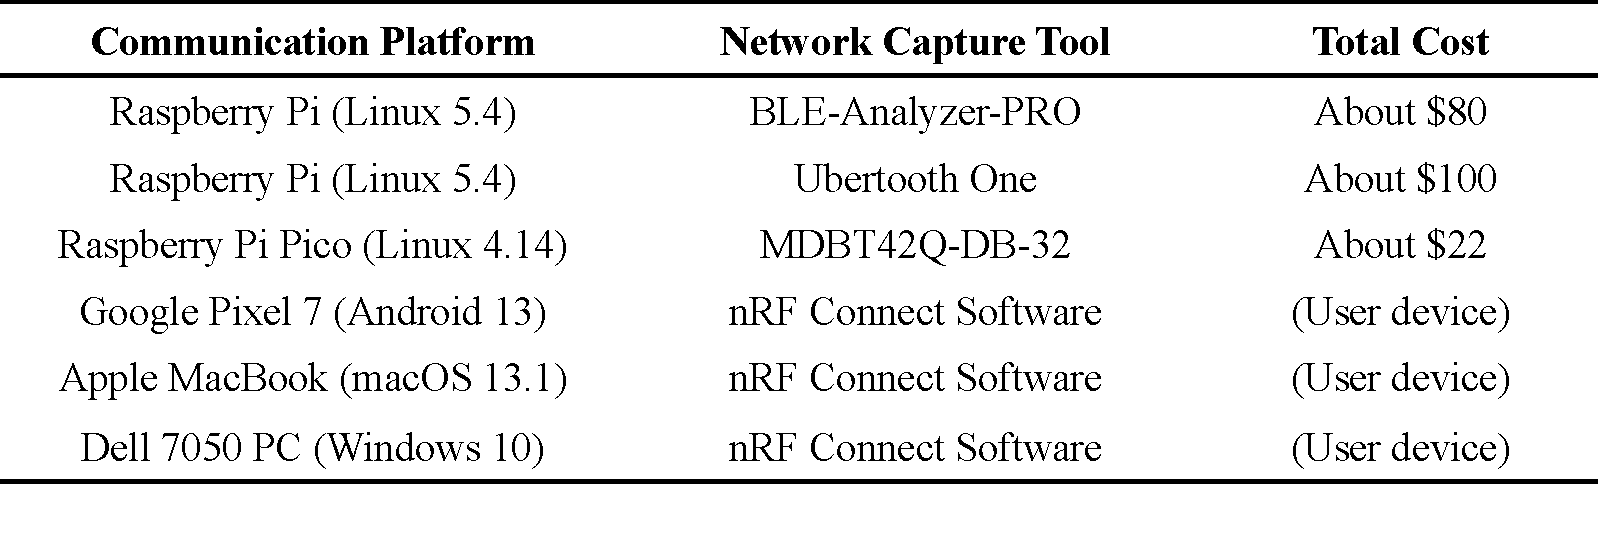
\includegraphics[width=1\linewidth]{FZU thesis templete//Table/appendices-1-4.pdf}
\end{figure}


% \begin{figure}[h]
%     \centering
%     \caption*{Appendices 1-2: Sample data of BLE packets recorded during the collecting phase.}
%     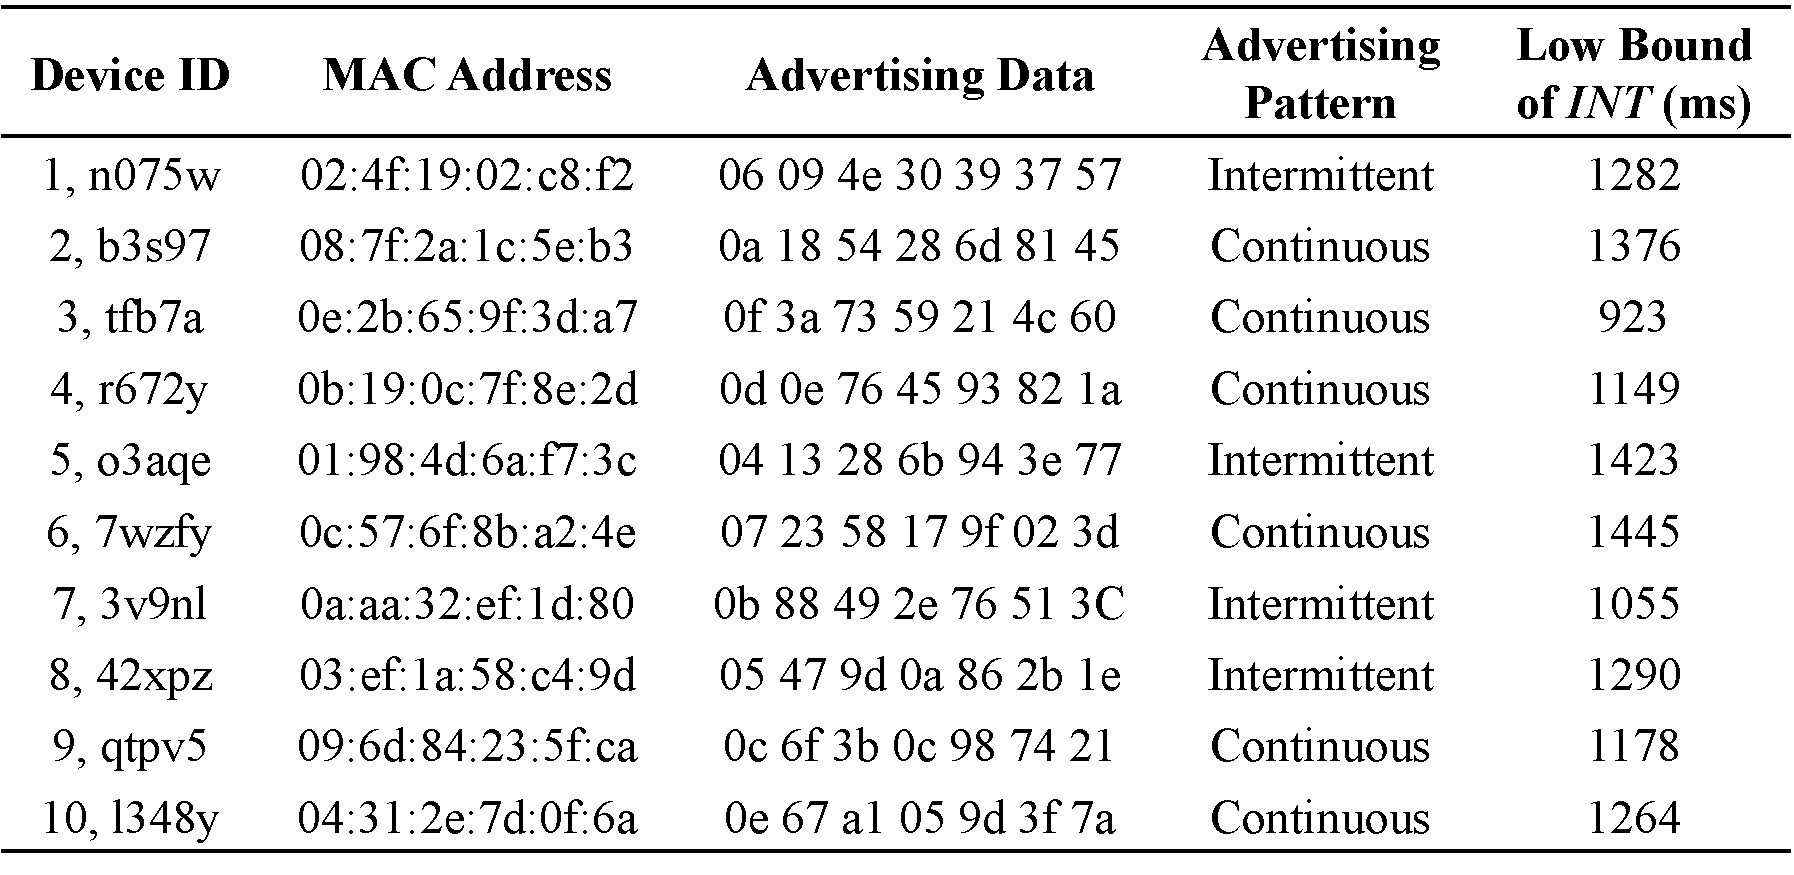
\includegraphics[width=1\linewidth]{FZU thesis templete//Table/appendices-1-5.pdf}
% \end{figure}

\vspace{48pt}

% ————————————————————————————————————————————————————————————————————— %
% ————————————————————————————————————————————————————————————————————— %


\subsection{Appendices 2: Related Publication for this Project}

\vspace{12pt}

\begin{enumerate}
    \item [{[1]}] Securing Billion Bluetooth Devices leveraging Learning-based Technique[C]. The 38th Annual AAAI Conference on Artificial Intelligence, undergraduate consortium (AAAI 2024, Research Proposal). \textbf{First Author}. Related to the Chapter 4 (4.2).
    \item [{[2]}] Hybrid Detection Mechanism for Spoofing Attacks in Bluetooth Low Energy Networks[C]. The 22nd ACM International Conference on Mobile Systems, Applications, and Services (MobiSys 2024, Poster). \textbf{First Author}. Related to the Chapter 4 (4.3).
\end{enumerate}

\vspace{4pt}

\noindent Please note that I am the first author of the publications included in this appendix, which closely relate to the work discussed in this report. Due to the inclusion of these paper and their overlap with the content of this report, there may be an elevated similarity index when this document undergoes plagiarism checks. This statement serves to declare that such similarities are expected and result from the reuse of foundational work from my own published research, contributing directly to the development of this project. This declaration is made to ensure transparency and to preclude any potential concerns regarding the originality of the work presented herein.

\vspace{8pt}

\begin{figure}[H]
    \centering
    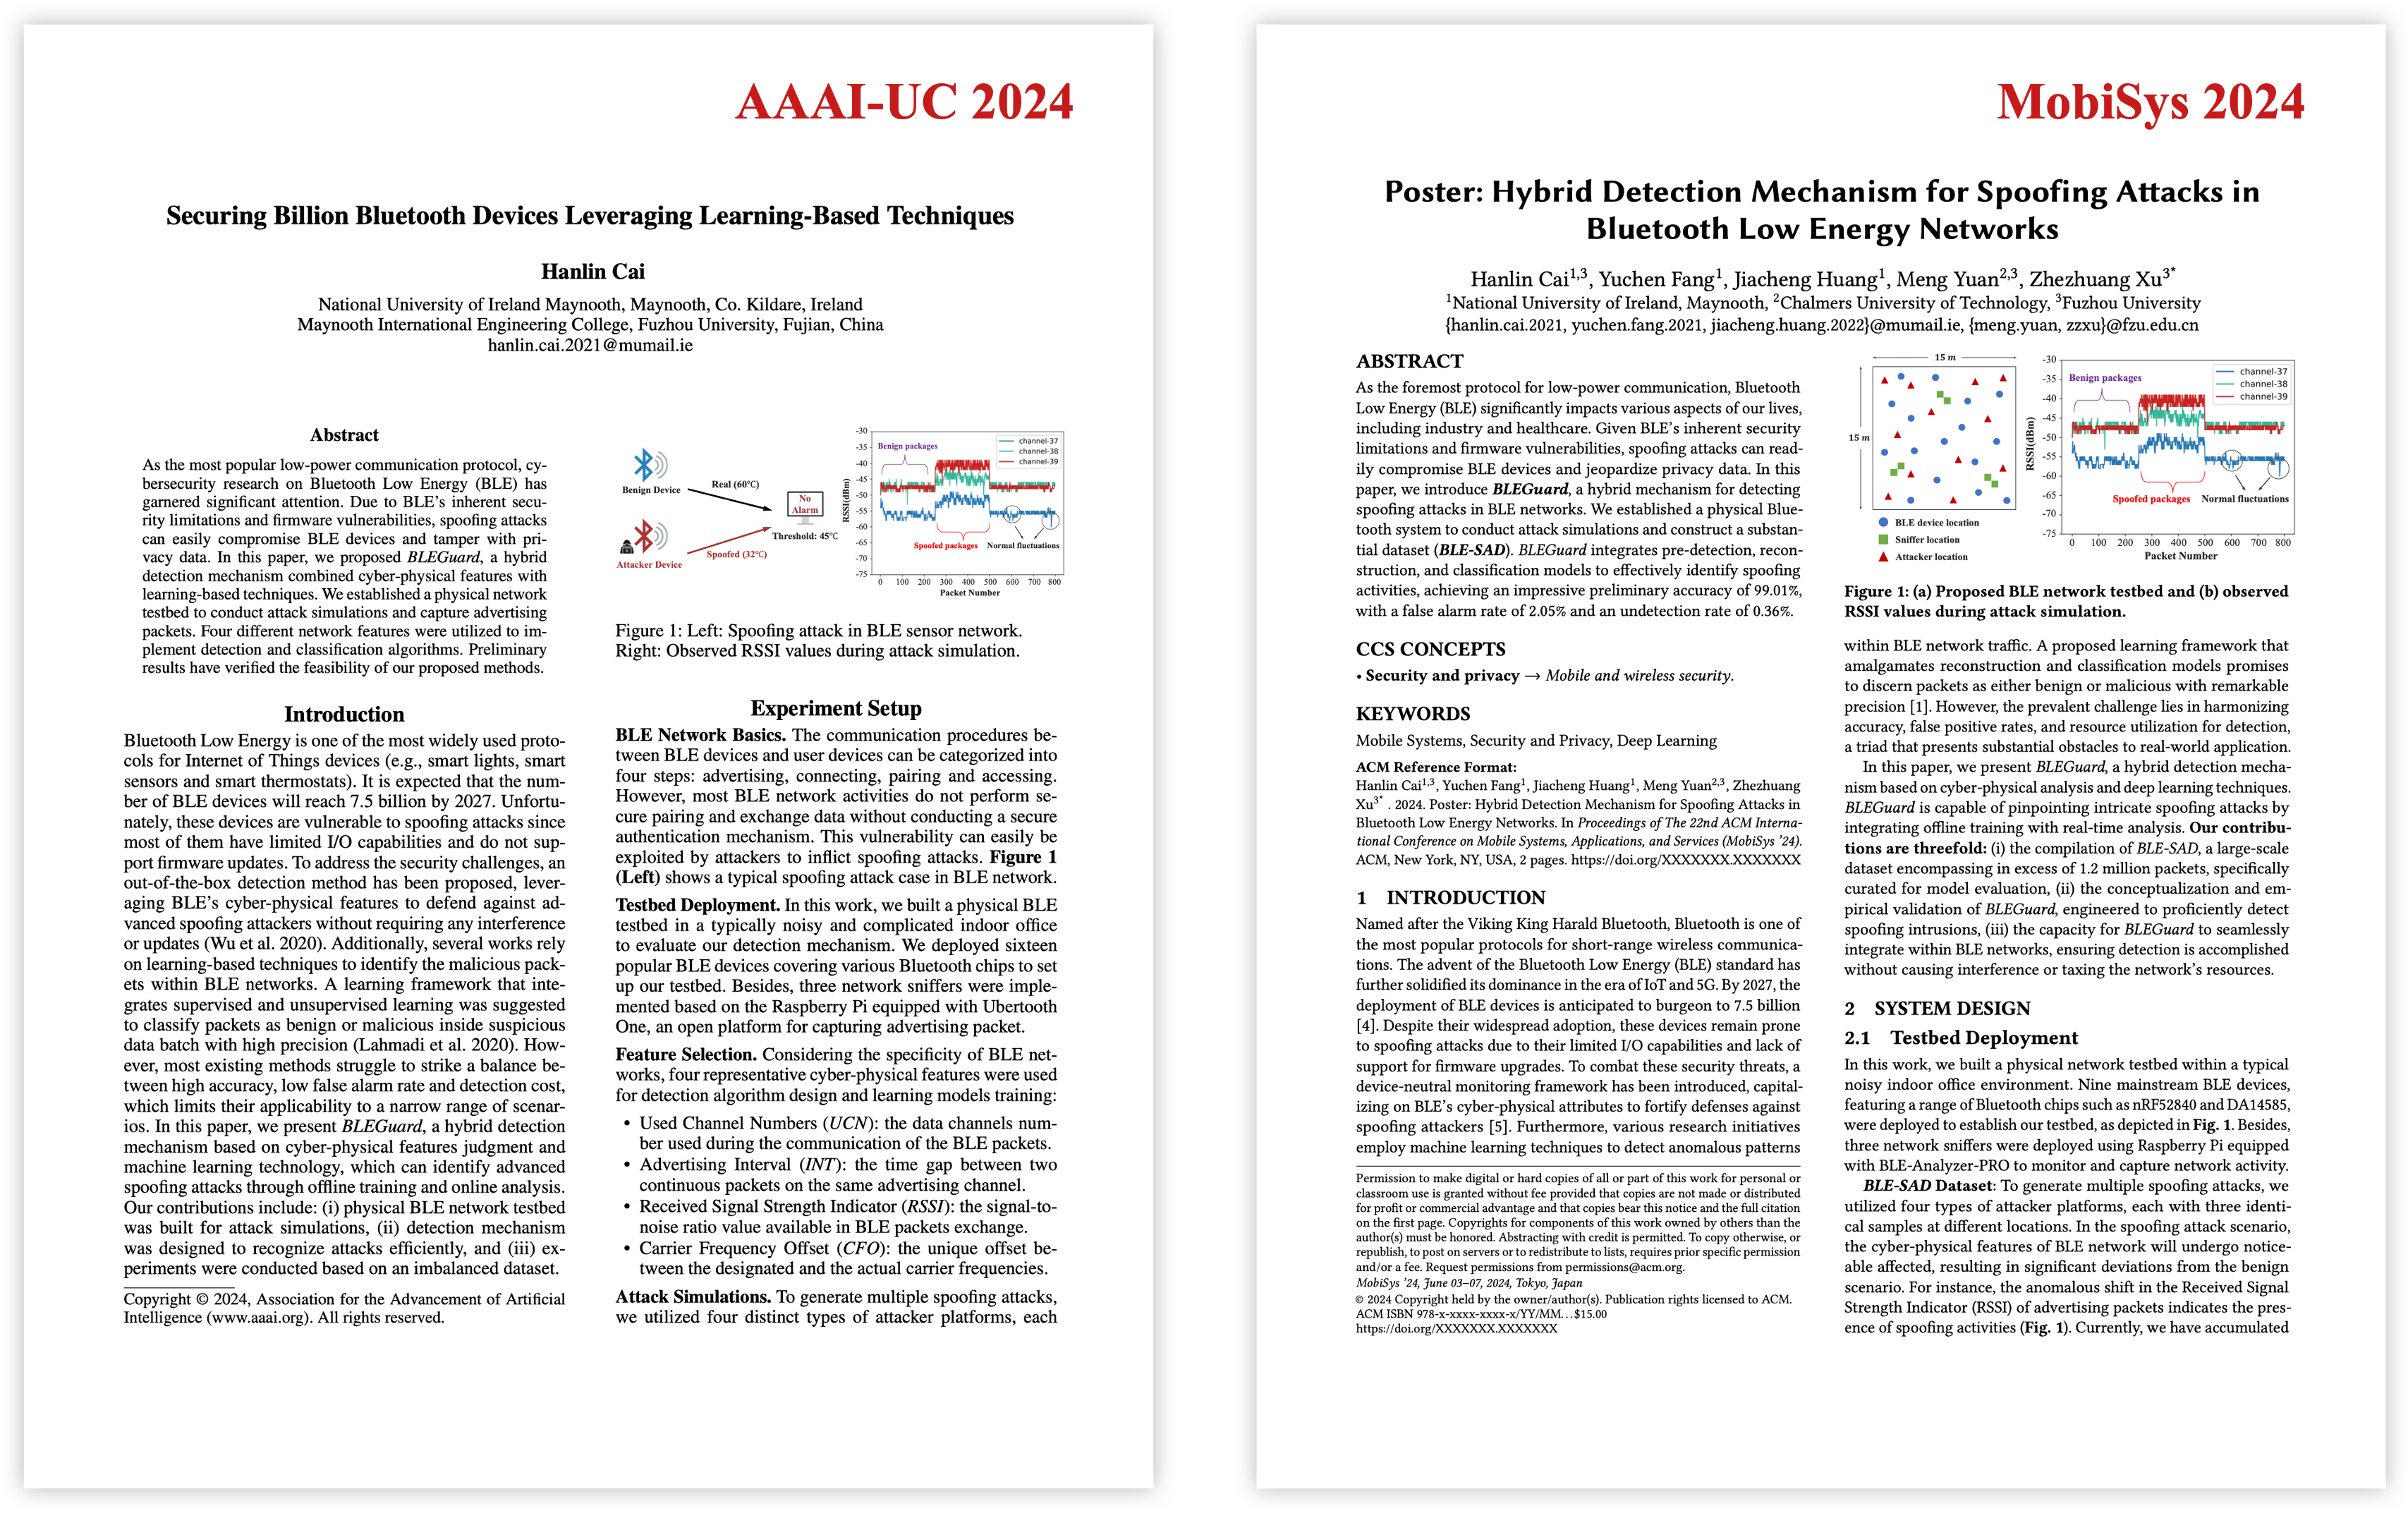
\includegraphics[width=1\linewidth]{FZU thesis templete/Fig/appendices-fig2.png}
    \caption*{Appendices 2-1: Related Publication for this Project}
\end{figure}


\newpage